\frame{
    \frametitle{New MC Samples!}
    \begin{columns} \begin{column}{0.5\textwidth}
        \begin{center} 
            619 Possible Combinations of 6,\\
            250 Include SM Sample

            \resizebox{0.3\textheight}{!}{\begin{tabular}{ |l|l|l| }
                \hline
                \textbf {$\kappa_{2V}$} & \textbf {$\kappa_\lambda$} & \textbf {$\kappa_V$} \\
                \hline
                0    & 0   & 1   \\
                0    & 1   & 1   \\
                0.5  & 1   & 1   \\
                1    & 0   & 1   \\
                1    & 1   & 0.5 \\
                1    & 1   & 1   \\
                1    & 1   & 1.5 \\
                1    & 10  & 1   \\
                1    & 2   & 1   \\
                1.5  & 1   & 1   \\
                2    & 1   & 1   \\
                3    & 1   & 1   \\
                \hline
            \end{tabular}}
        \end{center}
    \end{column} \begin{column}{0.5\textwidth}
        {\footnotesize Rank combinations by the surface integral of the number of negative bins at each point at in the $\kappa$ parameter space (mutliplying by the $\kvv \times \kl$ ``area" of each square)}

        \begin{figure}
        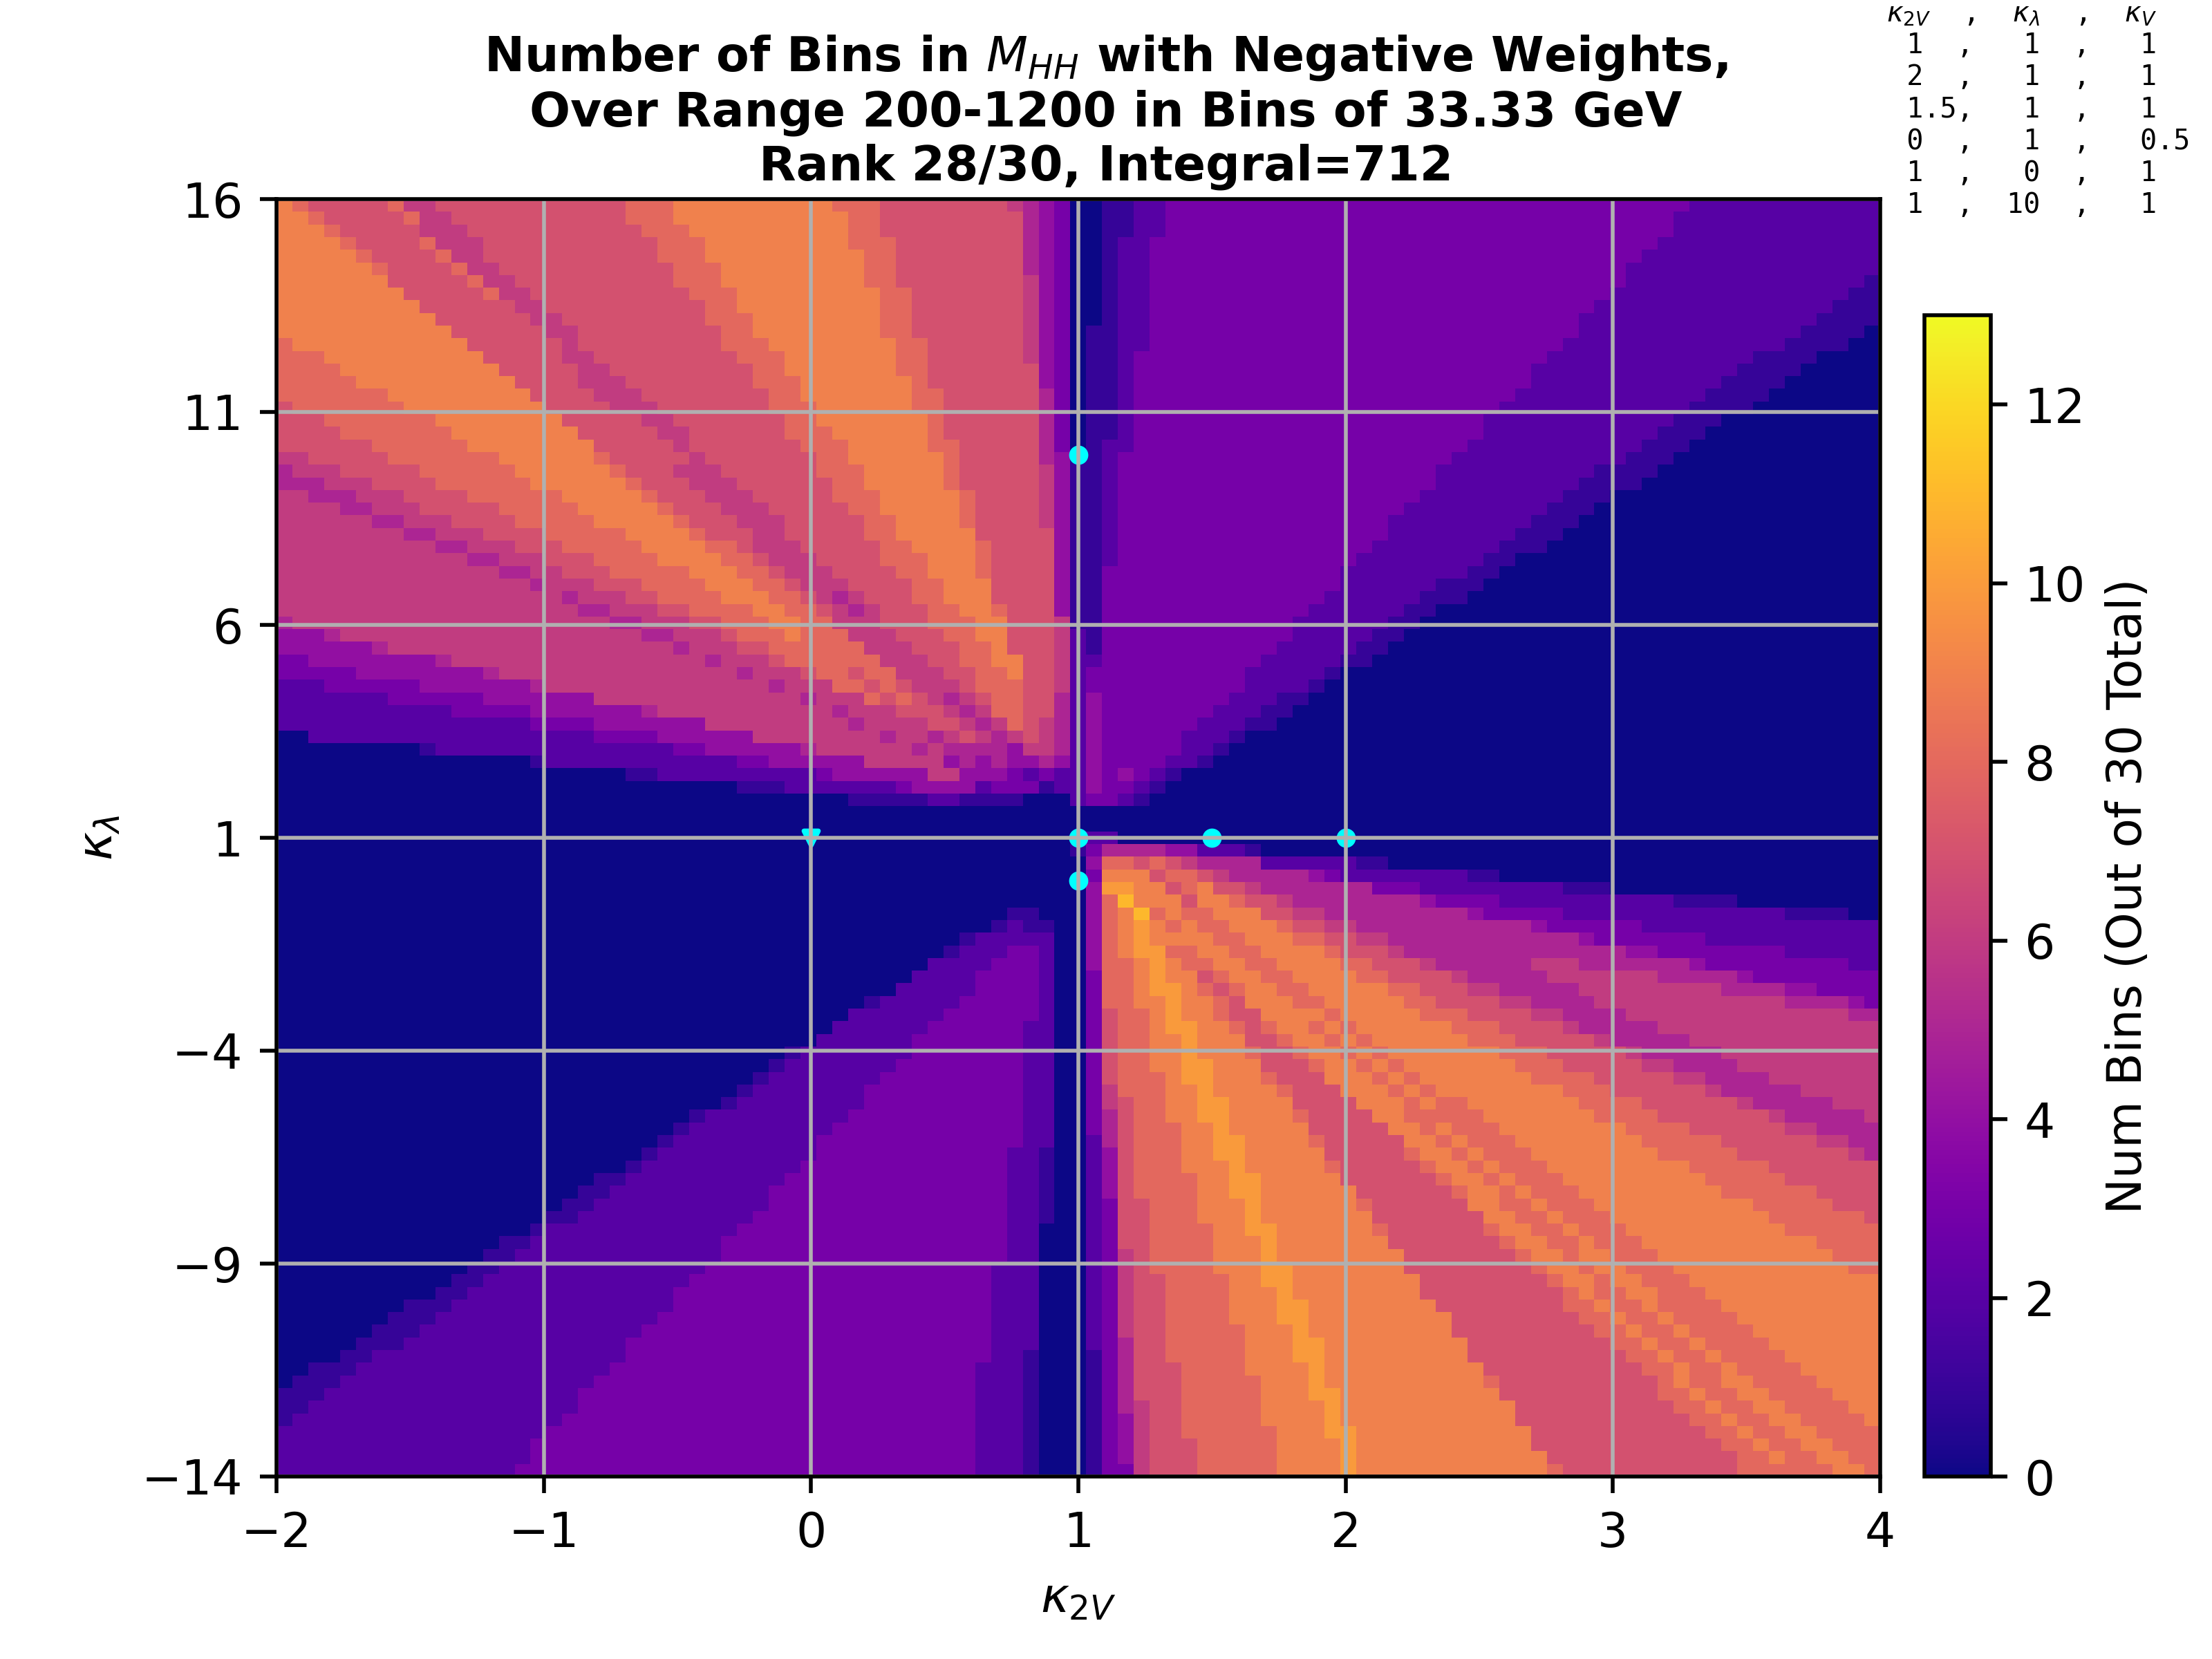
\includegraphics[width=\linewidth,height=\textheight,keepaspectratio]{negative_weights_rank027}
        \end{figure}

         {\tiny All plots produced using ``cryptotuple" MC samples.}
    \end{column} \end{columns}
}
